\clearpage
\textbf{High Traffic Scenario:}\\

As this scenario is quite complex the model was taking a long time to obtain a result and therefore a deadline has been set. This deadline was one week (7 days) because we assume that at this time it is possible to find an optimal solution.
In a first phase, we will show the resulting physical and optical topology. These topologies are based on the allowed topologies referred to in the model description and also taking into account the logical topology for all ODUs mentioned in the section \ref{high_traffic_scenario}. \\

\begin{figure}[h!]
\centering
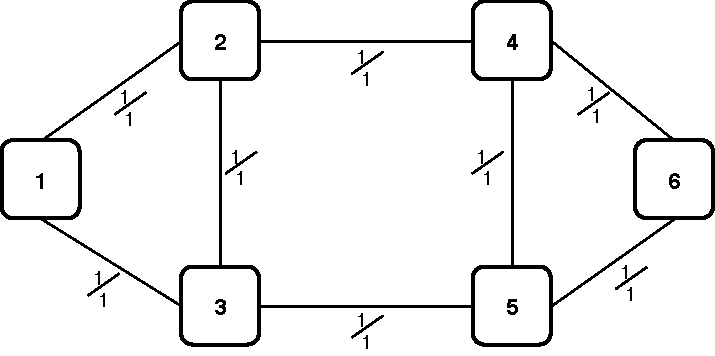
\includegraphics[width=11cm]{sdf/ilp/translucent_protection/figures/physical_topology}
\caption{Translucent with 1+1 protection in high scenario: physical topology after dimensioning.}
\label{physical3_protectionhigh}
\end{figure}

\begin{figure}[h!]
\centering
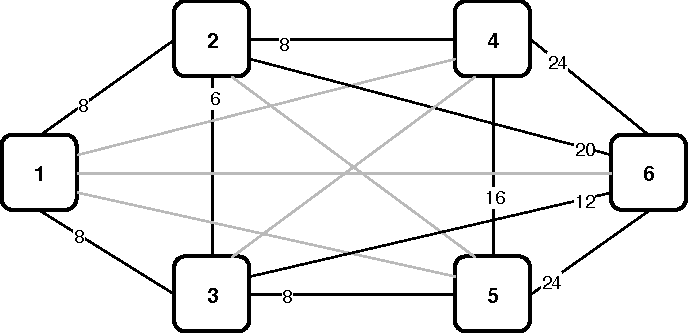
\includegraphics[width=11cm]{sdf/ilp/translucent_protection/figures/optical_topology_high}
\caption{Translucent with 1+1 protection in high scenario: optical topology after dimensioning.}
\label{optical3_protectionhigh}
\end{figure}

In table \ref{link_transluc_protec_ref_high} we can see the number of optical channels calculated using \ref{Capex_Link} and \ref{ILPOpaque_CAPEX} and the number of amplifiers for each link calculated using \ref{Capex_amplifiers}.\\

In table \ref{node_transluc_protec_ref_high} we can see the resulting nodal degree at the physical layer, the number of line ports and add ports using \ref{OXC_poxc_transluc} the number of long-reach transponders using \ref{EXC_pexc2_transluc} and the number of tributary ports using \ref{EXC_pexc1_transluc}.\\
\newpage
\begin{table}[h!]
\centering
\begin{tabular}{|| c | c | c ||}
 \hline
 \multicolumn{3}{|| c ||}{Information regarding links} \\
 \hline
 \hline
 Bidirectional Link & Optical Channels & Amplifiers\\
 \hline
 Node 1 <-> Node 2 & 8 & 4 \\
 Node 1 <-> Node 3 & 8 & 6 \\
 Node 2 <-> Node 3 & 6 & 0 \\
 Node 2 <-> Node 4 & 28 & 6 \\
 Node 3 <-> Node 5 & 20 & 8 \\
 Node 4 <-> Node 5 & 16 & 1 \\
 Node 4 <-> Node 6 & 44 & 7 \\
 Node 5 <-> Node 6 & 36 & 3 \\
 \hline
\end{tabular}
\caption{Table with information regarding links for translucent mode with 1+1 protection in high scenario.}
\label{link_transluc_protec_ref_high}
\end{table}

\begin{table}[h!]
\centering
\begin{tabular}{|| c | c | c | c | c | c ||}
 \hline
 \multicolumn{6}{|| c ||}{Information regarding nodes} \\
 \hline
 \hline
 \multicolumn{2}{|| c |}{ } & \multicolumn{2}{ c |}{Electrical part} & \multicolumn{2}{ c ||}{Optical part} \\
 \hline
 Node & Resulting Nodal Degree & Tributary Ports & LR Transponders & Add Ports & Line Ports\\
 \hline
 1 & 2 & 580 & 16 & 16 & 16 \\
 2 & 3 & 460 & 42 & 42 & 42 \\
 3 & 3 & 360 & 34 & 34 & 34 \\
 4 & 3 & 400 & 48 & 48 & 88 \\
 5 & 3 & 480 & 48 & 48 & 72 \\
 6 & 2 & 440 & 80 & 80 & 80 \\
\hline
\end{tabular}
\caption{Table with information regarding nodes for translucent mode with 1+1 protection in high scenario.}
\label{node_transluc_protec_ref_high}
\end{table}

Through the information obtained previously on the nodes we can now create tables with detailed information about each node.

\begin{table}[h!]
\centering
\begin{tabular}{|| c | c | c ||}
 \hline
 \multicolumn{3}{|| c ||}{Detailed description of Node 1} \\
 \hline
 \hline
 Electrical part & Number of total demands & Bit rate \\
 \hline
\multirow{3}{*}{580 tributary ports} & 260 & ODU0 \\
 & 260 & ODU1 \\
 & 60 & ODU2 \\
 \hline
  & Node<--Optical Channels-->Node & Bit rate \\
 \hline
\multirow{2}{*}{16 LR Transponders} & 1  <---- 8 ---->  2 & \multirow{2}{*}{100 Gbits/s} \\
  & 1  <---- 8 ---->  3 & \\
 \hline
 \hline
 Optical part & Node<--Optical Channels-->Node & Bit rate \\
 \hline
 \multirow{2}{*}{16 add ports} & 1  <---- 8 ---->  2 & \multirow{4}{*}{100 Gbits/s} \\
  & 1  <---- 8 ---->  3 & \\ \cline{1-2}
 \multirow{2}{*}{16 line ports} & 1  <---- 8 ---->  2 & \\
  & 1  <---- 8 ---->  3 & \\
\hline
\end{tabular}
\caption{Translucent with 1+1 protection in high scenario: detailed description of node 1. The number of demands is distributed to the various destination nodes, this distribution can be observed in section \ref{high_traffic_scenario}.}
\end{table}
\newpage
\begin{table}[h!]
\centering
\begin{tabular}{|| c | c | c ||}
 \hline
 \multicolumn{3}{|| c ||}{Detailed description of Node 2} \\
 \hline
 \hline
 Electrical part & Number of total demands & Bit rate \\ \hline
\multirow{5}{*}{460 tributary ports} & 220 & ODU0 \\
 & 140 & ODU1 \\
 & 40 & ODU2 \\
 & 40 & ODU3 \\
 & 20 & ODU4 \\
 \hline
  & Node<--Optical Channels-->Node & Bit rate \\
  \hline
\multirow{4}{*}{42 LR Transponders} & 2  <---- 8 ---->  1 & \multirow{4}{*}{100 Gbits/s} \\
  & 2  <---- 6 ---->  3 & \\
  & 2  <---- 8 ---->  4 & \\
  & 2  <---- 20 ---->  6 & \\
 \hline
 \hline
 Optical part & Node<--Optical Channels-->Node & Bit rate \\
 \hline
 \multirow{4}{*}{42 add ports} & 2  <---- 8 ---->  1 & \multirow{8}{*}{100 Gbits/s} \\
  & 2  <---- 6 ---->  3 & \\
  & 2  <---- 8 ---->  4 & \\
  & 2  <---- 20 ---->  6 & \\ \cline{1-2}
 \multirow{4}{*}{42 line ports} & 2  <---- 8 ---->  1 & \\
  & 2  <---- 6 ---->  3 & \\
  & 2  <---- 8 ---->  4 & \\
  & 2  <---- 20 ---->  6 & \\
\hline
\end{tabular}
\caption{Translucent with 1+1 protection in high scenario: detailed description of node 2. The number of demands is distributed to the various destination nodes, this distribution can be observed in section \ref{high_traffic_scenario}.}
\end{table}

\begin{table}[h!]
\centering
\begin{tabular}{|| c | c | c ||}
 \hline
 \multicolumn{3}{|| c ||}{Detailed description of Node 4} \\
 \hline
 \hline
 Electrical part & Number of total demands & Bit rate \\ \hline
\multirow{3}{*}{400 tributary ports} & 140 & ODU0 \\
 & 200 & ODU1 \\
 & 60 & ODU2 \\
 \hline
  & Node<--Optical Channels-->Node & Bit rate \\ \hline
 \multirow{3}{*}{48 LR Transponders} & 4  <---- 8 ---->  2 & \multirow{3}{*}{100 Gbits/s} \\
  & 4  <---- 16 ---->  5 & \\
  & 4  <---- 24 ---->  6 & \\
 \hline
 \hline
 Optical part & Node<--Optical Channels-->Node & Bit rate \\
 \hline
 \multirow{3}{*}{48 add ports} & 4  <---- 8 ---->  2 & \multirow{7}{*}{100 Gbits/s} \\
  & 4  <---- 16 ---->  5 & \\
  & 4  <---- 24 ---->  6 & \\ \cline{1-2}
 \multirow{4}{*}{88 line ports} & 4  <---- 8 ---->  2 & \\
  & 4  <---- 16 ---->  5 & \\
  & 4  <---- 24 ---->  6 & \\
  & 2  <---- 20 ---->  6 & \\
\hline
\end{tabular}
\caption{Translucent with 1+1 protection in high scenario: detailed description of node 4. The number of demands is distributed to the various destination nodes, this distribution can be observed in section \ref{high_traffic_scenario}.}
\end{table}

\newpage
\begin{table}[h!]
\centering
\begin{tabular}{|| c | c | c ||}
 \hline
 \multicolumn{3}{|| c ||}{Detailed description of Node 3} \\
 \hline
 \hline
 Electrical part & Number of total demands & Bit rate \\
 \hline
 \multirow{4}{*}{360 tributary ports} & 140 & ODU0 \\
 & 120 & ODU1\\
 & 60 & ODU2\\
 & 40 & ODU3\\
 \hline
  & Node<--Optical Channels-->Node & Bit rate \\ \hline
 \multirow{4}{*}{34 LR Transponders} & 3  <---- 8 ---->  1 & \multirow{4}{*}{100 Gbits/s} \\
  & 3  <---- 6 ---->  2 & \\
  & 3  <---- 8 ---->  5 & \\
  & 3  <---- 12 ---->  6 & \\
 \hline
 \hline
 Optical part & Node<--Optical Channels-->Node & Bit rate \\
 \hline
 \multirow{4}{*}{34 add ports} & 3  <---- 8 ---->  1 & \multirow{8}{*}{100 Gbits/s} \\
  & 3  <---- 6 ---->  2 & \\
  & 3  <---- 8 ---->  5 & \\
  & 3  <---- 12 ---->  6 & \\ \cline{1-2}
 \multirow{4}{*}{34 line ports} & 3  <---- 8 ---->  1 & \\
  & 3  <---- 6 ---->  2 & \\
  & 3  <---- 8 ---->  5 & \\
  & 3  <---- 12 ---->  6 & \\
\hline
\end{tabular}
\caption{Translucent with 1+1 protection in high scenario: detailed description of node 3. The number of demands is distributed to the various destination nodes can be observed in section \ref{high_traffic_scenario}.}
\end{table}

\begin{table}[h!]
\centering
\begin{tabular}{|| c | c | c ||}
 \hline
 \multicolumn{3}{|| c ||}{Detailed description of Node 5} \\
 \hline
 \hline
 Electrical part & Number of total demands & Bit rate \\ \hline
\multirow{5}{*}{480 tributary ports} & 280 & ODU0 \\
 & 80 & ODU1 \\
 & 80 & ODU2 \\
 & 20 & ODU3 \\
 & 20 & ODU4 \\
 \hline
  & Node<--Optical Channels-->Node & Bit rate \\ \hline
 \multirow{3}{*}{48 LR Transponders} & 5  <---- 8 ---->  3 & \multirow{3}{*}{100 Gbits/s} \\
  & 5  <---- 16 ---->  4 & \\
  & 5  <---- 24 ---->  6 & \\
 \hline
 \hline
 Optical part & Node<--Optical Channels-->Node & Bit rate \\
 \hline
 \multirow{3}{*}{24 add ports} & 5  <---- 8 ---->  3 & \multirow{7}{*}{100 Gbits/s} \\
  & 5  <---- 16 ---->  4 & \\
  & 5  <---- 24 ---->  6 & \\ \cline{1-2}
 \multirow{4}{*}{72 line ports} & 5  <---- 8 ---->  3 & \\
  & 5  <---- 16 ---->  4 & \\
  & 5  <---- 24 ---->  6 & \\
  & 3  <---- 12 ---->  6 & \\
\hline
\end{tabular}
\caption{Translucent with 1+1 protection in high scenario: detailed description of node 5. The number of demands is distributed to the various destination nodes can be observed in section \ref{high_traffic_scenario}.}
\end{table}

\newpage
\begin{table}[h!]
\centering
\begin{tabular}{|| c | c | c ||}
 \hline
 \multicolumn{3}{|| c ||}{Detailed description of Node 6} \\
 \hline
 \hline
 Electrical part & Number of total demands & Bit rate \\ \hline
\multirow{5}{*}{440 tributary ports} & 160 & ODU0 \\
 & 200 & ODU1 \\
 & 20 & ODU2 \\
 & 20 & ODU3 \\
 & 40 & ODU4 \\
 \hline
  & Node<--Optical Channels-->Node & Bit rate \\ \hline
 \multirow{4}{*}{80 LR Transponders} & 6  <---- 20 ---->  2 & \multirow{4}{*}{100 Gbits/s} \\
  & 6  <---- 12 ---->  3 & \\
  & 6  <---- 24 ---->  4 & \\
  & 6  <---- 24 ---->  5 & \\
 \hline
 Optical part & Node<--Optical Channels-->Node & Bit rate \\
 \hline
 \multirow{4}{*}{80 add ports} & 6  <---- 20 ---->  2 & \multirow{8}{*}{100 Gbits/s} \\
  & 6  <---- 12 ---->  3 & \\
  & 6  <---- 24 ---->  4 & \\
  & 6  <---- 24 ---->  5 & \\ \cline{1-2}
 \multirow{4}{*}{80 line ports} & 6  <---- 20 ---->  2 & \\
  & 6  <---- 12 ---->  3 & \\
  & 6  <---- 24 ---->  4 & \\
  & 6  <---- 24 ---->  5 & \\
\hline
\end{tabular}
\caption{Translucent with 1+1 protection in high scenario: detailed description of node 6. The number of demands is distributed to the various destination nodes can be observed in section \ref{high_traffic_scenario}.}
\end{table}

On the next page we have the table with the routing information where once more the paths are bidirectional.
Finally in the table \ref{scripttransluc_protec_ref_high} we have the CAPEX result for this model.
\begin{table}[h!]
\centering
\begin{tabular}{||c|c|c|c|c|c|c||}
 \hline
 \multicolumn{7}{||c||}{CAPEX of the Network} \\
 \hline
 \hline
 \multicolumn{3}{||c|}{}&Quantity&Unit Price&Cost&Total \\
 \hline
 \multirow{3}{*}{\makecell{Link \\ Cost}}&\multicolumn{2}{c|}{OLTs}&16&15 000 \euro&240 000 \euro&\multirow{3}{*}{166 520 000 \euro}\\ \cline{2-6}
 &\multicolumn{2}{c|}{100 Gbits/s Transceivers}&332&5 000 \euro/Gbit/s&166 000 000 \euro&\\ \cline{2-6}
 &\multicolumn{2}{c|}{Amplifiers}&70&4 000 \euro&280 000 \euro& \\
 \hline
 \multirow{10}{*}{\makecell{Node \\ Cost}}&\multirow{7}{*}{Electrical}&EXCs&6&10 000 \euro&60 000 \euro&\multirow{10}{*}{28 531 800 \euro} \\ \cline{3-6}
 & &ODU0 Ports&1 200&10 \euro/port&12 000 \euro& \\ \cline{3-6}
 & &ODU1 Ports&1 000&15 \euro/port&15 000 \euro& \\ \cline{3-6}
 & &ODU2 Ports&320&30 \euro/port&9 600 \euro& \\ \cline{3-6}
 & &ODU3 Ports&120&60 \euro/port&7 200 \euro& \\ \cline{3-6}
 & &ODU4 Ports&80&100 \euro/port&8 000 \euro& \\ \cline{3-6}
 & &Transponders&268&100 000 \euro/port&26 800 000 \euro& \\ \cline{2-6}
 &\multirow{3}{*}{Optical}&OXCs&6&20 000 \euro&120 000 \euro&\\ \cline{3-6}
 & &Line Ports&332&2 500 \euro/port&830 000 \euro& \\ \cline{3-6}
 & &Add Ports&268&2 500 \euro/port&670 000 \euro& \\
 \hline
 \multicolumn{6}{||c|}{Total Network Cost}&195 051 800 \euro\\
\hline
\end{tabular}
\caption{Translucent with 1+1 protection in high scenario: detailed description of CAPEX for this scenario.}
\label{scripttransluc_protec_ref_high}
\end{table}

\newpage
\begin{table}[h]
\centering
\begin{tabular}{||c|c|c|c|c||}
 \hline
 \multicolumn{5}{|| c ||}{Routing} \\
 \hline
 \hline
 o & d & Type & Links & Demands \\
 \hline
 \multirow{2}{*}{1}&\multirow{2}{*}{2}&W&\{(1,3),(3,5),(5,6),(6,4),(4,2)\}&100 ODU0, 40 ODU1, 20 ODU2\\
  & &P& \{(1,2)\} &100 ODU0, 40 ODU1, 20 ODU2 \\ \hline
 \multirow{2}{*}{1}&\multirow{2}{*}{3}&W& \{(1,2),(2,3)\} & 20 ODU0, 80 ODU1, 20 ODU2\\
  & &P& \{(1,3)\} & 20 ODU0, 80 ODU1, 20 ODU2 \\ \hline
 \multirow{2}{*}{1} & \multirow{2}{*}{4}&W&\{(1,3),(3,5),(5,6),(6,4)\}&60 ODU0, 40 ODU1, 20 ODU2\\
  & &P& \{(1,2),(2,4)\} & 60 ODU0, 40 ODU1, 20 ODU2 \\ \hline
 \multirow{2}{*}{1} & \multirow{2}{*}{5}&W&\{(1,2),(2,4),(4,5)\}& 20 ODU0\\
  & &P& \{(1,3),(3,5)\} & 20 ODU0 \\ \hline
 \multirow{2}{*}{1} & \multirow{2}{*}{6}&W& \{(1,3),(3,5),(5,6)\} & 60 ODU0, 100 ODU1 \\
  & &P& \{(1,2),(2,4),(4,6)\} & 60 ODU0, 100 ODU1 \\ \hline
 \multirow{5}{*}{2} & \multirow{5}{*}{3}&W& \{(2,1),(1,3)\} & 10 ODU3 \\
  & &W& \{(2,4),(4,6),(6,5),(5,3)\} & 7 ODU3 \\
  & &W& \{(2,3)\} & 3 ODU3 \\
  & &P& \{(2,3)\} & 12 ODU3 \\
  & &P& \{(2,1),(1,3)\} & 8 ODU3 \\ \hline
 \multirow{2}{*}{2} & \multirow{2}{*}{4}&W&\{(2,4),(4,6),(6,4)\}&20 ODU0, 60 ODU1 \\
  & &P& \{(2,4)\} & 20 ODU0, 60 ODU1 \\ \hline
 \multirow{4}{*}{2} & \multirow{4}{*}{5}&W&\{(2,4),(4,5)\} & 100 ODU0, 20 ODU1 \\
  & &W& \{(2,1),(1,3),(3,5)\} & 20 ODU2 \\
  & &P& \{(2,3),(3,5)\} & 100 ODU0, 20 ODU1 \\
  & &P& \{(2,4),(4,5)\} & 20 ODU2 \\ \hline
 \multirow{4}{*}{2} & \multirow{4}{*}{6}&W&\{(2,3),(3,5),(5,6)\}& 20 ODU1, 6 ODU4 \\
  & &W& \{(2,4),(4,6)\} & 20 0DU3, 8 ODU4 \\
  & &W& \{(2,1),(1,3),(3,5),(5,6)\} & 6 ODU4 \\
  & &P& \{(2,4),(4,6)\} & 20 ODU1, 20 ODU3, 20 ODU4 \\ \hline
 \multirow{2}{*}{3} & \multirow{2}{*}{4}&W& \{(3,5),(5,6),(6,4)\} & 20 ODU0, 20 ODU1, 20 ODU2 \\
  & &P& \{(3,2),(2,4)\} & 20 ODU0, 20 ODU1, 20 ODU2 \\ \hline
 \multirow{3}{*}{3}&\multirow{3}{*}{5}&W&\{(3,2),(2,4),(4,5)\}&80 ODU0, 20 ODU1 \\
  & &W& \{(3,5),(5,6),(6,4),(4,5)\}& 20 ODU2, 20 ODU3\\
  & &P& \{(3,5)\} & 80 ODU0, 20 ODU1, 20 ODU2, 20 ODU3 \\ \hline
 \multirow{2}{*}{3} & \multirow{2}{*}{6}&W& \{(3,2),(2,4),(4,6)\} & 20 ODU0 \\
  & &P& \{(3,6)\} & 20 ODU0 \\ \hline
 \multirow{3}{*}{4} & \multirow{3}{*}{5}&W& \{(4,2),(2,3),(3,5)\} & 20 ODU0 \\
  & &W& \{(4,6),(6,5),(5,3),(3,5)\} & 20 ODU1, 20 ODU2 \\
  & &P& \{(4,5)\} & 20 ODU0, 20 ODU1, 20 ODU2 \\ \hline
 \multirow{2}{*}{4} & \multirow{2}{*}{6}&W& \{(4,2),(2,4),(4,6)\} & 20 ODU0, 60 ODU1\\
  & &P& \{(4,6)\} & 20 ODU0, 60 ODU1\\ \hline
 \multirow{3}{*}{5} & \multirow{3}{*}{6}&W&\{(5,3),(3,5),(5,6)\}& 60 ODU0, 20 ODU1, 20 ODU2, 4 ODU4 \\
  & &W& \{(5,4),(4,6)\} & 16 ODU4 \\
  & &P& \{(5,6)\}& 60 ODU0, 20 ODU1, 20 ODU2, 20 ODU4 \\ \hline
\end{tabular}
\caption{Translucent with 1+1 protection in high scenario: description of demands routing. The type W means that it is working path and type P protection path.}
\label{path_transluc_protec_ref_high}
\end{table}
\newpage
